\NativeTitle{1}{第一单元素养评价（A）}{（四则混合运算）}{40}{5}{一 & 二 & 三 & 四 & 五}{ &  &  &  & }
% Page 1 body. Each NativeSlot uses original portrait coordinates in bp.
\def\OrigTop#1{\vtop{\hrule width0pt height0pt\hbox{#1}}}
% p001_s01
\NativeSlot{278}{66}{%
  {\heiti 一、填空。}（第3～7题每题2分，其余各题每空1分，共24分）\par
  1.\quad 添加括号使\(671+29\times4\div2\)的运算顺序变为先求和，再求积，最后求商，则原\par
  \hspace*{1.45em}式变为（\hspace{170bp}）。\par
}
% p001_s02
% p001_s03
\NativeSlot{355}{27}{%
  2.\quad 先在\(\square\)里填上合适的数，再列出综合算式。\par
}
\NativeSlot{384}{94}{%
  \noindent\hbox to \linewidth{%
    \hbox to 282bp{\hskip18bp\OrigTop{（1）}\hskip7bp%
      \OrigTop{\resizebox{!}{90bp}{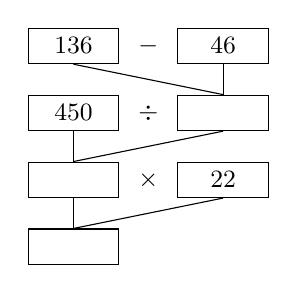
\begin{tikzpicture}[x=1cm,y=1cm,every node/.style={font=\small},b/.style={draw,minimum width=1.15cm,minimum height=.45cm}]\node[b] (n00) at (0.0,0.0) {\(136\)};\node[b] (n01) at (1.9,0.0) {\(46\)};\node at (.95,0.0) {$-$};\node[b] (n10) at (0.0,-0.85) {\(450\)};\node[b] (n11) at (1.9,-0.85) {};\node at (.95,-0.85) {$\div$};\draw (n00.south)--(n11.north);\draw (n01.south)--(n11.north);\node[b] (n20) at (0.0,-1.7) {};\node[b] (n21) at (1.9,-1.7) {\(22\)};\node at (.95,-1.7) {$\times$};\draw (n10.south)--(n20.north);\draw (n11.south)--(n20.north);\node[b] (n30) at (0.0,-2.55) {};\draw (n20.south)--(n30.north);\draw (n21.south)--(n30.north);\end{tikzpicture}
}}\hfil}%
    \hskip18bp\OrigTop{（2）}\hskip7bp%
    \OrigTop{\resizebox{!}{90bp}{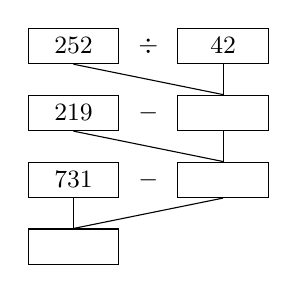
\begin{tikzpicture}[x=1cm,y=1cm,every node/.style={font=\small},b/.style={draw,minimum width=1.15cm,minimum height=.45cm}]\node[b] (n00) at (0.0,0.0) {\(252\)};\node[b] (n01) at (1.9,0.0) {\(42\)};\node at (.95,0.0) {$\div$};\node[b] (n10) at (0.0,-0.85) {\(219\)};\node[b] (n11) at (1.9,-0.85) {};\node at (.95,-0.85) {$-$};\draw (n00.south)--(n11.north);\draw (n01.south)--(n11.north);\node[b] (n20) at (0.0,-1.7) {\(731\)};\node[b] (n21) at (1.9,-1.7) {};\node at (.95,-1.7) {$-$};\draw (n10.south)--(n21.north);\draw (n11.south)--(n21.north);\node[b] (n30) at (0.0,-2.55) {};\draw (n20.south)--(n30.north);\draw (n21.south)--(n30.north);\end{tikzpicture}
}}\hfil}%
}
\NativeSlot{488}{25}{%
  \noindent\hbox to \linewidth{\hskip18bp 综合算式：\rule{136bp}{.4bp}。%
    \hfil 综合算式：\rule{136bp}{.4bp}。}\par
}
% p001_s04
\NativeSlot{513}{45}{%
  3.\quad 根据运算顺序，把\(53-35=18\)、\(18\times4=72\)、\(720\div72=10\)改写成综合算式是\par
  \hspace*{1.45em}（\hspace{172bp}）。\par
}
% p001_s05
\NativeSlot{566}{22}{%
  4.\quad 要使\(8\times(\square\div5)=120\)，\(\square\)里应填（\hspace{2.25em}）。\par
}
% p001_s06
\NativeSlot{592}{49}{%
  5.\quad 小丽在计算一道除法算式时，把除数\(32\)看成了\(23\)，算出来的商是\(34\)，余数是\par
  \hspace*{1.45em}\(18\)。这道计算题正确的结果是（\hspace{2.25em}）。\par
}
% p001_s07
% p001_s08
\NativeSlot{646}{78}{%
  6.\quad 在\(\bigcirc\)里填上“\(>\)”“\(<\)”或“\(=\)”。\par
  \vspace{5bp}%
  \hspace*{1.45em}\(122\times40-15+328\ \bigcirc\ 122\times(40-15)+328\)\par
  \vspace{5bp}%
  \hspace*{1.45em}\(560\div(14-6)\times5\ \bigcirc\ 560\div[(14-6)\times5]\)\par
}
% p001_s09
\NativeSlot{730}{68}{%
  \noindent\hbox to \linewidth{%
    \begin{minipage}[t]{295bp}\vspace{0pt}%
      7.\quad 傍晚，王叔叔在小区里走路锻炼，步行\(2\)分钟\par
      \hspace*{1.45em}后，他手机计步 APP 显示如图。照这样计算，\par
    \end{minipage}\hfill
    \OrigTop{\begin{tikzpicture}[x=1bp,y=1bp,font=\small,inner sep=0pt]
      \draw[black,line width=.55bp] (30,30) circle[radius=29];
      \draw[black,line width=.5bp] (30,30) circle[radius=24];
      \draw[black,line width=.5bp] (30,54)--(30,59) (54,30)--(59,30);
      \node at (30,29) {\(200\)步};
      \node at (90,39) {步行距离};
      \node at (90,22) {\(130\)米};
      \node at (149,39) {消耗热量};
      \node at (149,22) {\(4\)千卡};
    \end{tikzpicture}}%
  }\par
}
